\documentclass[a4paper,12pt]{report}
\usepackage[table]{xcolor}
\usepackage[T1]{fontenc}
\usepackage[utf8]{inputenc}
\usepackage[greek,english]{babel}
\usepackage{geometry}
\usepackage{amsmath}
\usepackage{graphicx}
\usepackage{hyperref}
\usepackage{caption}
\usepackage{subcaption}
\usepackage{wrapfig}
\usepackage{tabularx}
\usepackage{booktabs}
\usepackage{multicol}
\usepackage{multirow}
\usepackage{listings}
\usepackage{xcolor}
\usepackage[export]{adjustbox}
\usepackage[most]{tcolorbox}
\captionsetup{justification=centering}
\geometry{left=2.5cm, right=2.5cm, top=2.5cm, bottom=2.5cm}


\setlength{\parindent}{0pt}
\renewcommand*{\familydefault}{\rmdefault}
\newcommand{\gr}{\selectlanguage{greek}}
\newcommand{\en}{\selectlanguage{english}}
\setlength{\arrayrulewidth}{0.4mm}

\definecolor{codegray}{rgb}{0.5,0.5,0.5}
\definecolor{codegreen}{rgb}{0,0.6,0}
\definecolor{codeblue}{rgb}{0,0,1}
\definecolor{babypink}{RGB}{255, 230, 240} % very soft pink
\definecolor{lightorange}{RGB}{255,240,220}
\definecolor{lightyellow}{RGB}{255, 255, 204}
\definecolor{babyblue}{RGB}{220, 240, 255}
\lstdefinestyle{mystyle}{
	backgroundcolor=\color{white},   
	commentstyle=\color{codegreen},
	keywordstyle=\color{codeblue},
	numberstyle=\tiny\color{codegray},
	stringstyle=\color{red},
	basicstyle=\ttfamily\footnotesize,
	breakatwhitespace=false,         
	breaklines=true,                 
	captionpos=b,                    
	keepspaces=true,                 
	numbers=left,                    
	numbersep=5pt,                  
	showspaces=false,                
	showstringspaces=false,
	showtabs=false,                  
	tabsize=4
}

\lstset{style=mystyle}
\lstset{
	backgroundcolor=\color{babyblue},
	basicstyle=\ttfamily\footnotesize,
	language=Python,
	showstringspaces=false,
	captionpos=b
}


\lstdefinestyle{mystyle}{
  basicstyle={\small\ttfamily},
  keywordstyle=\color{blue},
  commentstyle=\color{green},
  numbers=left,
  numberstyle=\tiny\color{gray}
}




\begin{document}

\begin{titlepage}
\begin{center}
  
\includegraphics[scale=0.5]{UOM.png}
\end{center}

{\vspace{2em}}
\begin{flushright}
    2024/25
\end{flushright}

\noindent
\framebox{%
    \begin{minipage}{1.0\linewidth} 
        \vspace{5pt} 
        \centering
        \begin{tabular}{ l @{\hspace{10pt}} l } 
            \textbf{\gr Κατζός Γεώργιος:} & \en ics22074 \\
            \textbf{\gr Γηρούση Ευαγγελία:} & \en ics22048 \\
            \textbf{\gr Τίτλος:} & \en Diabetic feet ulcer monitoring \\
            \textbf{\gr Υπεύθυνος Καθηγητής:} & \gr Ευτύχιος Πρωτοπαπαδάκης \\
        \end{tabular}
        \vspace{5pt} % Adds space at the bottom
    \end{minipage}
}


\

{\vspace{7em}}

\centering
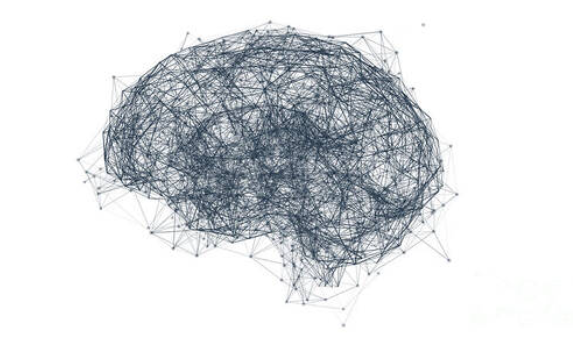
\includegraphics[scale=0.8]{neural.png}

{\vspace{5em}}

\begin{center}
  \Large{{\textbf{\gr Εφαρμοσμένη Πληροφορική}}}
\end{center}

{\medskip}

\begin{center}
  \gr Πανεπιστήμιο Μακεδονίας
\end{center}
\end{titlepage}
\gr                           
\tableofcontents
\gr
\chapter{\gr Προσδιορισμός και Κατανόηση του Προβλήματος}
\section{\gr Περιγραφή του Προβλήματος}
\paragraph{\textnormal{
\gr Τα διαβητικά έλκη ποδιών \en(Diabetic foot ulcer - DFU) \gr είναι μια σοβαρή και ευρέως διαδεδομένη επιπλοκή του διαβήτη, η οποία συντελεί σε μεγάλο βαθμό στη νοσηρότητα των ασθενών. Τα \en \textbf{DFUs} \gr εμφανίζονται εξαιτίας της κακής κυκλοφορίας του αίματος και της νευροπάθειας, με αποτέλεσμα την εμφάνιση χρόνιων τραυμάτων που είναι ιδιαίτερα ευαίσθητα στη μόλυνση. Οι έρευνες δείχνουν ότι περίπου το 15\% των διαβητικών ασθενών είναι πιθανό να αναπτύξουν έλκος στο πόδι κατά τη διάρκεια της ζωής τους, ενώ από την άλλη πλευρά το 85\% των ακρωτηριασμών των κάτω άκρων που συνδέονται με τον διαβήτη προέρχονται από μη θεραπεύμισα ή κακώς διαχειριζόμενα έλκη \cite{wagner2022}.}}
\paragraph{\textnormal{
\gr Ανεξαρτήτως των προόδων στην ιατρική θεραπεία των \en \textbf{DFUs}, \gr η έγκαιρη διάγνωση και η διαρκής παρακολούθηση εξακολουθούν να αποτελούν σημαντικές προκλήσεις. Η παραδοσιακή μέθοδος ανίχνευσης είναι χειροκίνητη και υποκειμενική, με αποτέλεσμα να παρατηρούνται συχνά διαγνωστικές ασυνέπειες. Επιπλέον, η απουσία εξειδικευμένης περίθαλψης σε απομακρυσμένες περιοχές έχει ως αποτέλεσμα την καθυστέρηση της θεραπείας, αυξάνοντας τον κίνδυνο επιπλοκών. Ως αποτέλεσμα, είναι επιτακτική η  ανάγκη για αυτοματοποιημένες, ακριβείς και επεκτάσιμες λύσεις για την πρόληψη, τη βελτίωση της ανίχνευσης και της διαχείρισης των \en \textbf{DFU}.
}}
\section{\gr Η Σημασία του Προβλήματος}
\paragraph{\textnormal{
\gr Τα \en \textbf{DFUs} \gr αποτελούν πρόβλημα για τα συστήματα υγειονομικής περίθαλψης λόγω των υψηλών ποσοστών υποτροπής που εμφανίζουν, της παρατεταμένης διάρκειας της θεραπείας τους και των επιπλοκών που σχετίζονται άμεσα με αυτά. Οι παραδοσιακές μέθοδοι αξιολόγησης και ταξινόμησης των \en \textbf{DFUs}, \gr όπως το σύστημα ταξινόμησης του \en Wagner, \gr στηρίζονται στην οπτική εξέταση και την κλινική κατάσταση του ασθενούς, γεγονός που ενδέχεται να έχει ως αποτέλεσμα ασυνέπεια και καθυστερήσεις στη θεραπεία \cite{dfu_classifications_review}.
}}
\paragraph{\textnormal{
\gr Επιπλέον, με την παρατεταμένη παραμονή στο νοσοκομείο λόγω των \en \textbf{DFUs} \gr και τις δαπανηρές ιατρικές πράξεις η οικονομική επιβάρυνση των παρόχων υγειονομικής περίθαλψης και των ασθενών αυξάνεται σημαντικά. Έρευνες επισημαίνουν ότι η έγκαιρη ανίχνευση και η έγκαιρη παρέμβαση δύναται να μειώσει αισθητά τα ποσοστά ακρωτηριασμών και το κόστος θεραπείας \cite{telemedical_monitoring}. Ωστόσο, εξακολουθεί να υπάρχει έλλειψη τυποποιημένων, αυτοματοποιημένων και κλιμακούμενων μεθόδων για την ανίχνευση και την παρακολούθηση των ελκών.
}}
\paragraph{\textnormal{
\gr Δεδομένων αυτών των προκλήσεων, η ενσωμάτωση της τεχνητής νοημοσύνης \en (AI) \gr και της βαθιάς μάθησης στην ανίχνευση των \en DFUs \gr αποτελεί μια ευοίωνη λύση. Τα διαγνωστικά εργαλεία με βάση την Τεχνητή Νοημοσύνη μπορούν να παρέχουν συνεπή και αποτελεσματική ανάλυση, μειώνοντας την εξάρτηση από τον ανθρώπινο παράγοντα και επιτρέπουν την παρακολούθηση εξ αποστάσεως, ιδίως για ασθενείς σε υποβαθμισμένες περιοχές.
}}
\section{\gr Πρόταση Λύσης}
\paragraph{\textnormal{
\gr Για να αντιμετωπιστούν οι περιορισμοί των παραδοσιακών μεθόδων ανίχνευσης των \en \textbf{DFUs}, \gr η παρούσα μελέτη προτείνει μια μέθοδο αυτοματοποιημένης ανίχνευσης και παρακολούθησης τους με τη χρήση της τεχνητής νοημοσύνης και πιο συγκεκριμένα μοντέλων βαθιάς μάθησης \en (Deep Learning). \gr Οι τεχνικές ανίχνευσης αντικειμένων, επιτρέπουν τον ακριβή εντοπισμό των ελκών εντός των εικόνων, επιτρέποντας την έγκαιρη διάγνωση και την σταδιακή παρακολούθηση με την πάροδο του χρόνου.
}}
\subsection{\gr Μεθοδολογία}
\paragraph{\textnormal{
\gr Tο προτεινόμενο σύστημα χρησιμοποιήει ένα σύνολο δεδομένων από εικόνες που εντοπίζονται \en \textbf{DFUs}. \gr Το σύνολο δεδομένων θα περιέχει εικόνες με επισημασμένες περιοχές έλκους, επιτρέποντας στο μοντέλο να μάθει πρότυπα για μελλοντική αποτελεσματική ανίχνευση. Το εκπαιδευμένο μοντέλο θα εφαρμοστεί για τον εντοπισμό περιοχών έλκους και την παρακολούθηση της εξέλιξης με την πάροδο του χρόνου.  Αυτό θα επιτρέψει τη συνεχή παρακολούθηση της επούλωσης των τραυμάτων και θα βοηθήσει τους κλινικούς γιατρούς στη λήψη αποφάσεων θεραπείας βάσει δεδομένων. 
}}
\subsection{\gr Η προσέγγιση της Ανίχνευσης Αντικειμένων (\en Object Detection)}
\paragraph{\textnormal{
\gr Σε αντίθεση με τα παραδοσιακά μοντέλα ταξινόμησης εικόνας που δύναται να προσδιορίσουν μόνο αν υπάρχει έλκος σε μια εικόνα, το συγκεκριμένο προσφέρει μια πιο ολοκληρωμένη λύση, καθώς όχι μόνο ανιχνεύει τα έλκη αλλά και τα εντοπίζει εντός των εικόνων. Με την χρήση των οριοθετημένων πλαισίων, τα μοντέλα ανίχνευσης αντικειμένων παρέχουν ακριβείς πληροφορίες αναφορικά με τις θέσεις των \en \textbf{DFUs}, \gr γεγονός που τα καθιστά ιδιαίτερα πολύτιμα για την παρακολούθηση της εξέλιξης της νόσου. Επιπλέον, o εντοπισμός αντικειμένων επιτρέπει την αυτοματοποιημένη μέτρηση του μεγέθους και του σχήματος του έλκους, η οποία είναι απαραίτητη για την χρονική εκτίμηση της επούλωσης του τραύματος.
}}
\gr 
\chapter{\gr Το Σύνολο Δεδομένων (\en Dataset)}
\section{\gr Περιγραφή του \en Dataset}
\paragraph{\textnormal{\gr Το \en \textbf{dataset} \gr που χρησιμοποιείται σε αυτό το έργο επικεντρώνεται στην ανίχνευση και τον εντοπισμό \en \textbf{DFUs}, \gr μέσω της χρήσης του \en \textbf{object detection}. \gr Αποκτήθηκε από το \en Roboflow Universe \cite{roboflow}, \gr μια πλατφόρμα που χρησιμοποιείται ευρέως για τη δημιουργία και τη διαχείριση \en dataset \gr υπολογιστικής όρασης \en (computer vision). \gr Το σύνολο δεδομένων, με τίτλο \en \textbf{Diabetic Foot Ulcer - v6}, \gr περιέχει 10.163 εικόνες, με \en \textbf{DFUs} \gr και έχει υποστεί \en \textbf{data augmentation} \gr για την ενίσχυση της γενικότητας και της αξιοπιστίας του μοντέλου ανίχνευσης, μέσω της χρήσης διαφορετικών σεναρίων.}}
\paragraph{\textnormal{\gr Κάθε εικόνα απεικονίζει ένα ανθρώπινο πόδι και συνοδεύεται από ένα \en \textbf{label} \gr σχετικό με  την παρουσία του διαβητικού έλκους, η οποία γίνεται αντιληπτή μέσω ενός οριοθετημένου πλαισίου \en (\textbf{bounding box}). \gr Οι σχολιασμοί παρέχονται σε πολλαπλές μορφές \en  (YOLO, COCO, Pascal VOC), \gr επιτρέποντας την υλοποιήση διαφορετικών μοντέλων μηχανικής μάθησης.}}
\section{\gr Περιγραφή Χαρακτηριστικών του \en Dataset}
\paragraph{\textnormal{\gr Στην παρούσα ενότητα παρουσιάζονται τα χαρακτηριστικά του \en \textbf{dataset}. \gr Τα δεδομένα αφορούν εικόνες με σχολιασμούς \en (\textbf{annotations}) \gr (Σχήμα 2.1) για την ανίχνευση των \en \textbf{DFUs}, \gr και είναι δυνατό να χρησιμοποιηθούν σε προβλήματα υπολογιστικής όρασης \en (\textbf{computer vision}). \gr Παρακάτω στον Πίνακα 2.1 αναλύονται τα δεδομένα μορφοποιημένα σύμφωνα με το πρότυπο \en (COCO format).\gr Ο αριθμός των εικόνων ισούται με 10.163, οι διαστάσεις της κάθε εικόνας είναι $640\times 640$ \en pixels \gr και τα χαρακτηριστικά \en (\textbf{features}) \gr της κάθε εγγραφής είναι 8.
\newline
}}
\begin{table}
\centering
\renewcommand{\arraystretch}{1.5}
\begin{tabular}{|>{\columncolor[HTML]{99CC66}}p{4cm}|>{\columncolor[HTML]{99CC66}}p{4cm}|>{\columncolor[HTML]{99CC66}}p{7cm}|}
\hline
\en\textbf{Name} & \en\textbf{Type} & \en\textbf{Description} \\ \hline

\rowcolor[HTML]{E6F2DA}
\en\textbf{Ulcer} & \en Categorical (0 or 1) & \gr Υποδεικνύει αν υπάρχει παρουσία διαβητικού έλκους. \gr Στην \en COCO \gr μορφή, η ύπαρξη του έλκους αντιστοιχεί στην κατηγορία με \en \textbf{id: 0}. \\ \hline

\rowcolor[HTML]{E6F2DA}
\en\textbf{File Name} & \en Categorical (String) & \gr Το όνομα του αρχείου εικόνας (π.χ. \en 100048.jpg\gr ), αποτελεί μοναδικό αναγνωριστικό κάθε εγγραφής. \\ \hline

\rowcolor[HTML]{E6F2DA}
\en\textbf{Image Width} & \en Integer & \gr Το οριζόντιο μέγεθος της εικόνας σε \en pixels\gr , σταθερά ορισμένο στα \en 640 pixels\gr . \\ \hline

\rowcolor[HTML]{E6F2DA}
\en\textbf{Image Height} & \en Integer & \gr Το κατακόρυφο μέγεθος της εικόνας σε \en pixels\gr , σταθερά ορισμένο στα \en 480 pixels\gr . \\ \hline

\rowcolor[HTML]{E6F2DA}
\en\textbf{Bounding Box X} & \en Float & \gr Η οριζόντια θέση του κέντρου του πλαισίου \en (bounding box) \gr που περιλαμβάνει το έλκος. \\ \hline

\rowcolor[HTML]{E6F2DA}
\en\textbf{Bounding Box Y} & \en Float & \gr Η κατακόρυφη θέση του κέντρου του πλαισίου \en (bounding box) \gr που περιλαμβάνει το έλκος. \\ \hline

\rowcolor[HTML]{E6F2DA}
\en\textbf{Bounding Box Width} & \en Float & \gr Το οριζόντιο μήκος του πλαισίου \en (bounding box) \gr που περιλαμβάνει το έλκος. \\ \hline

\rowcolor[HTML]{E6F2DA}
\en\textbf{Bounding Box Height} & \en Float & \gr Το κατακόρυφο μήκος του πλαισίου \en (bounding box) \gr που περιλαμβάνει το έλκος. \\ \hline

\rowcolor[HTML]{E6F2DA}
\en\textbf{Split} & \en Categorical (String) & \gr Ο διαχωρισμός των εικόνων σε σύνολο εκπαίδευσης \en (train)\gr , επικύρωσης \en (val)\gr , ή ελέγχου \en (test)\gr . \\ \hline

\end{tabular}
\caption{\gr \textbf{Πίνακας Μεταβλητών και Χαρακτηριστικών}}
\end{table}

\begin{minipage}{0.4\textwidth}
	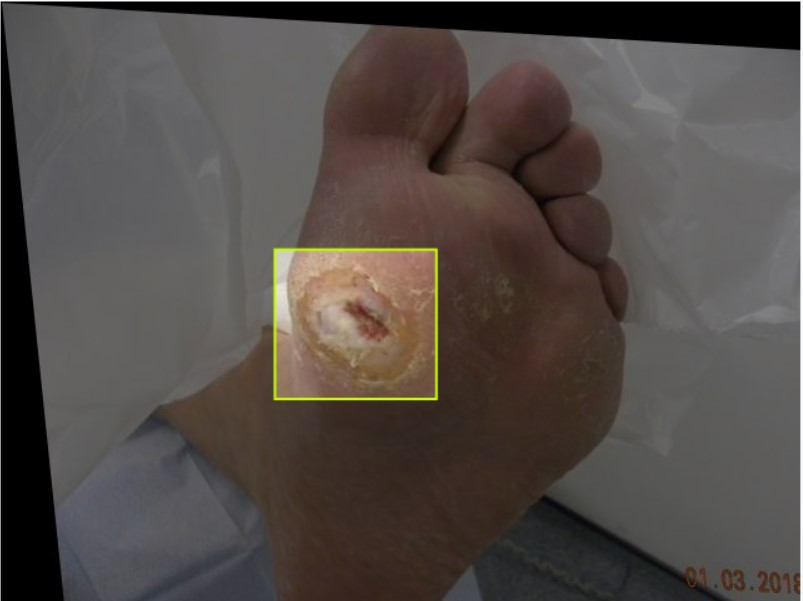
\includegraphics[width=0.85\textwidth, right]{100330.jpg}
\end{minipage}
\hfill
\begin{minipage}{0.5\textwidth}
	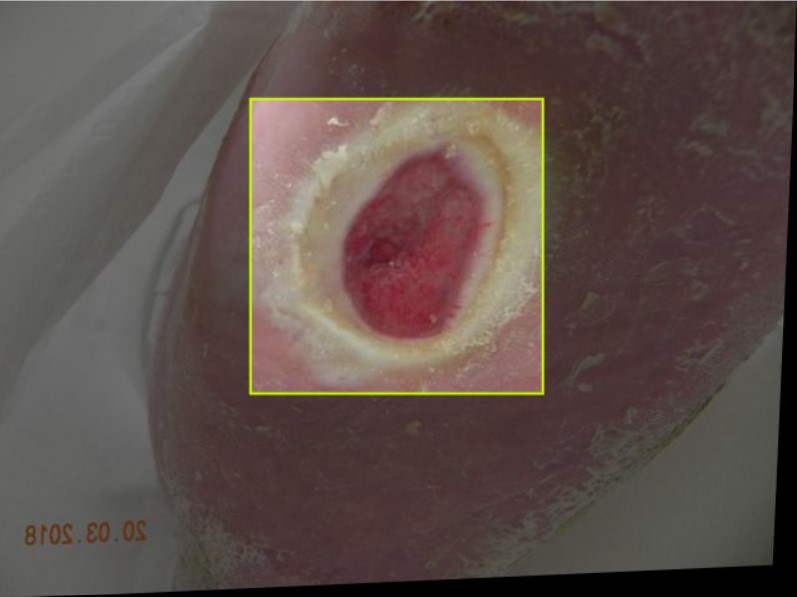
\includegraphics[width=0.7\textwidth, right]{100382.jpg}
	
\end{minipage}
\gr 
\captionof{figure}{\gr Εικόνες από το σύνολο δεδομένων \en Diabetic Foot Ulcer \gr με σημειωμένα έλκη για χρήση σε εφαρμογές ιατρικής ανάλυσης εικόνας.}

\section{\gr Λόγοι Επιλογής του \en Dataset}
\paragraph{\textnormal{\gr Το συγκεκριμένο \en \textbf{dataset} \gr επιλέχθηκε για την παρούσα εργασία για μια σειρά από λόγους που σχετίζονται τόσο με την ποιότητα όσο και με τη συνάφειά του με το πρόβλημα της ανίχνευσης ελκών σε ασθενείς με διαβήτη. Πιο συγκεκριμένα, κατέχει:}}
\begin{enumerate}
    \item \gr \textbf{\underline{Ιατρική Σημασία:}} Τα \en \textbf{DFUs} \gr αποτελούν σοβαρή επιπλοκή για ασθενείς με σακχαρώδη διαβήτη, καθώς μπορούν να οδηγήσουν σε ακρωτηριασμό αν δεν εντοπιστούν έγκαιρα. Το συγκεκριμένο \en \textbf{dataset} \gr επιτρέπει την εκπαίδευση μοντέλων, τα οποία θα δύναται να συμβάλλουν στην πρώιμη διάγνωση.
    \item \gr \textbf{\underline{Ποιότητα Σχολιασμών:}} Οι σχολιασμοί \en (\textbf{annotations}) \gr έχουν πραγματοποιηθεί με ακρίβεια, με τη χρήση αναγνωρισμένων προτύπων (\en YOLO \gr και \en COCO).
    \item \gr \textbf{\underline{\en Augmentation:}} \gr Το ενσωματωμένο \en \textbf{augmentation} \gr ενισχύει τη γενίκευση των μοντέλων που θα υλοποιηθούν.
    \item \gr \textbf{\underline{Ανοιχτή Πρόσβαση:}} Το \en \textbf{dataset} \gr διατίθεται δημόσια, γεγονός που επιτρέπει την ελεύθερη χρήση, τροποποίηση και δημοσίευση αποτελεσμάτων.
    \item \gr \textbf{\underline{Δομή:}} Το \en \textbf{dataset} \gr έχει σαφώς καθορισμένη δομή, με ελάχιστα έως καθόλου κενά δεδομένα \en (\textbf{null}), \gr καθιστώντας το εύκολο να αναλυθεί και να επεκταθεί μελλοντικά.
\end{enumerate}
\chapter{\gr Προ-επεξεργασία Δεδομένων}
\paragraph{\textnormal{\gr  Η διαδικασία προ-επεξεργασίας των δεδομένων αποτελεί απαραίτητο στάδιο στην ανάπτυξη κάθε αλγορίθμου μηχανικής μάθησης και ειδικότερα σε εφαρμογές \en \textbf{object detection}, \gr όπως για παράδειγμα το \en YOLOv8 \cite{ultralytics} \gr που χρησιμοποιήθηκε στην παρούσα εργασία. Είναι σημαντικό να αναφερθεί ότι η ακρίβεια και η συνέπεια των δεδομένων διαδραματίζει πρωταγωνιστικό ρόλο στην τελική απόδοση του μοντέλου.}}

\section{\gr Ανάλυση και Διαχωρισμός Δεδομένων}
\paragraph{\textnormal{\gr Αρχικά, το \en \textbf{dataset} \gr ήταν διαχωρισμένο σε \en \textbf{training} \gr και \en \textbf{validation} \gr σύνολα. Καθώς απαιτούνταν και \en \textbf{test set}, \gr ενοποιήθηκαν όλα τα δεδομένα και πραγματοποιήθηκε νέα διαίρεση. Η διαδικασία επαναλαμβάνεται για κάθε \en \textbf{fold} \gr στο πλαίσιο της διασταυρούμενης επικύρωσης \en (\textbf{cross-validation}).}}

\section{\gr Μετατροπή \en Annotations}
\paragraph{\textnormal{\gr Τα δεδομένα λήφθηκαν από την ιστοσελίδα του \en \textbf{Roboflow} \gr στο κατάλληλο \en \textbf{format} \gr τύπου \en \textbf{COCO}. \gr Το \en \textbf{dataset} \gr υπό κανονικές συνθήκες θα περιείχε μία μόνο κατηγορία αντικειμένου, τα έλκη \en (\textbf{ulcers}). \gr Κατά τη λήψη, υπήρχε επιπλέον μια κατηγορία "0" που δεν αντιστοιχούσε σε καμία εικόνα, οπότε και αφαιρέθηκε.}}

\section{\gr Κανονικοποίηση Εικόνων και Διαστάσεις}
\paragraph{\textnormal{\gr Όλες οι εικόνες αναπροσαρμόστηκαν στο σταθερό μέγεθος των $640\times640$ \en pixels \gr με χρήση \en \textbf{padding} \gr και \en \textbf{resize}, \gr διαδικασία που υποστηρίζεται εσωτερικά από το \en \textbf{YOLOv8} \gr κατά το \en \textbf{training}. \gr Η τυποποίηση αυτή διευκολύνει τη σύγκριση αποτελεσμάτων μεταξύ διαφορετικών μοντέλων και διασφαλίζει ότι η πληροφορία αξιοποιείται ισότιμα.}}

\section{Διαχωρισμός Εισόδων και Ετικετών}
\paragraph{\textnormal{\gr Καθώς πρόκειται για πρόβλημα εντοπισμού αντικειμένων \en (\textbf{object detection}), \gr κάθε δείγμα (εικόνα) συνδέεται με μία ή περισσότερες ετικέτες \en (bounding boxes \gr με κλάσεις). Η είσοδος προς το μοντέλο είναι μία εικόνα, ενώ η έξοδος είναι οι συντεταγμένες και τα \en bounding boxes \gr των αντικειμένων. Τα δεδομένα οργανώνονται αυτόματα μέσω του \en YAML, \gr το οποίο είναι αρχείο ρύθμισης που καθορίζει τη διαδρομή είτε για \en\textbf{ train}, \gr είτε για \en \textbf{validation} \gr είτε για \en \textbf{test}.}}

\chapter{\gr Διερεύνηση Δεδομένων}
\paragraph{\textnormal{\gr Η διερεύνηση δεδομένων αποτελεί το επόμενο στάδιο αυτής της μελέτης και έχει ως σκοπό την αποτύπωση της ποιότητας, της κατανομής και των συσχετίσεων στα δεδομένα. Στο πλαίσιο της παρούσας εργασίας, όπου χρησιμοποιούνται εικόνες και σημειώσεις \en \textbf{bounding boxes} \gr για ανίχνευση διαβητικών ελκών, η διερεύνηση περιλαμβάνει:}}
\begin{itemize}
    \item \gr Ανάλυση της πληρότητας και της ορθότητας των \en annotations.
    \item \gr Κατανομή της ύπαρξης \en DFU \gr ανά εικόνα.
    \item \gr Σύγκριση του \en \textbf{ground truth} \gr με τα \en \textbf{predicted bounding boxes}.
    \item \gr Στατιστικά ανά \en \textbf{fold cross-validation}.
\end{itemize}
\section{\gr Η Κατανομή των \en Bounding Boxes}
\paragraph{\textnormal{
\gr Κατά τη διερεύνηση του \en \textbf{dataset} \gr εντοπίστηκαν συνολικά 10.163 εικόνες, στις οποίες τα \en DFUs \gr έχουν επισημανθεί με \en \textbf{bounding boxes}. \gr Η κλάση \en ulcer \gr είναι \en categorical (class\_id: 0). \gr Δεν εντοπίστηκαν εικόνες χωρίς αντίστοιχο \en \textbf{label}, \gr γεγονός που επιβεβαιώνει τη συνέπεια του \en \textbf{dataset}. \gr Η κατανομή των ετικετών ήταν ισορροπημένη μεταξύ \en \textbf{training} \gr και \en \textbf{validation set} \gr (Σχήμα 4.1).
\newline
}}
\begin{minipage}{0.4\textwidth}
	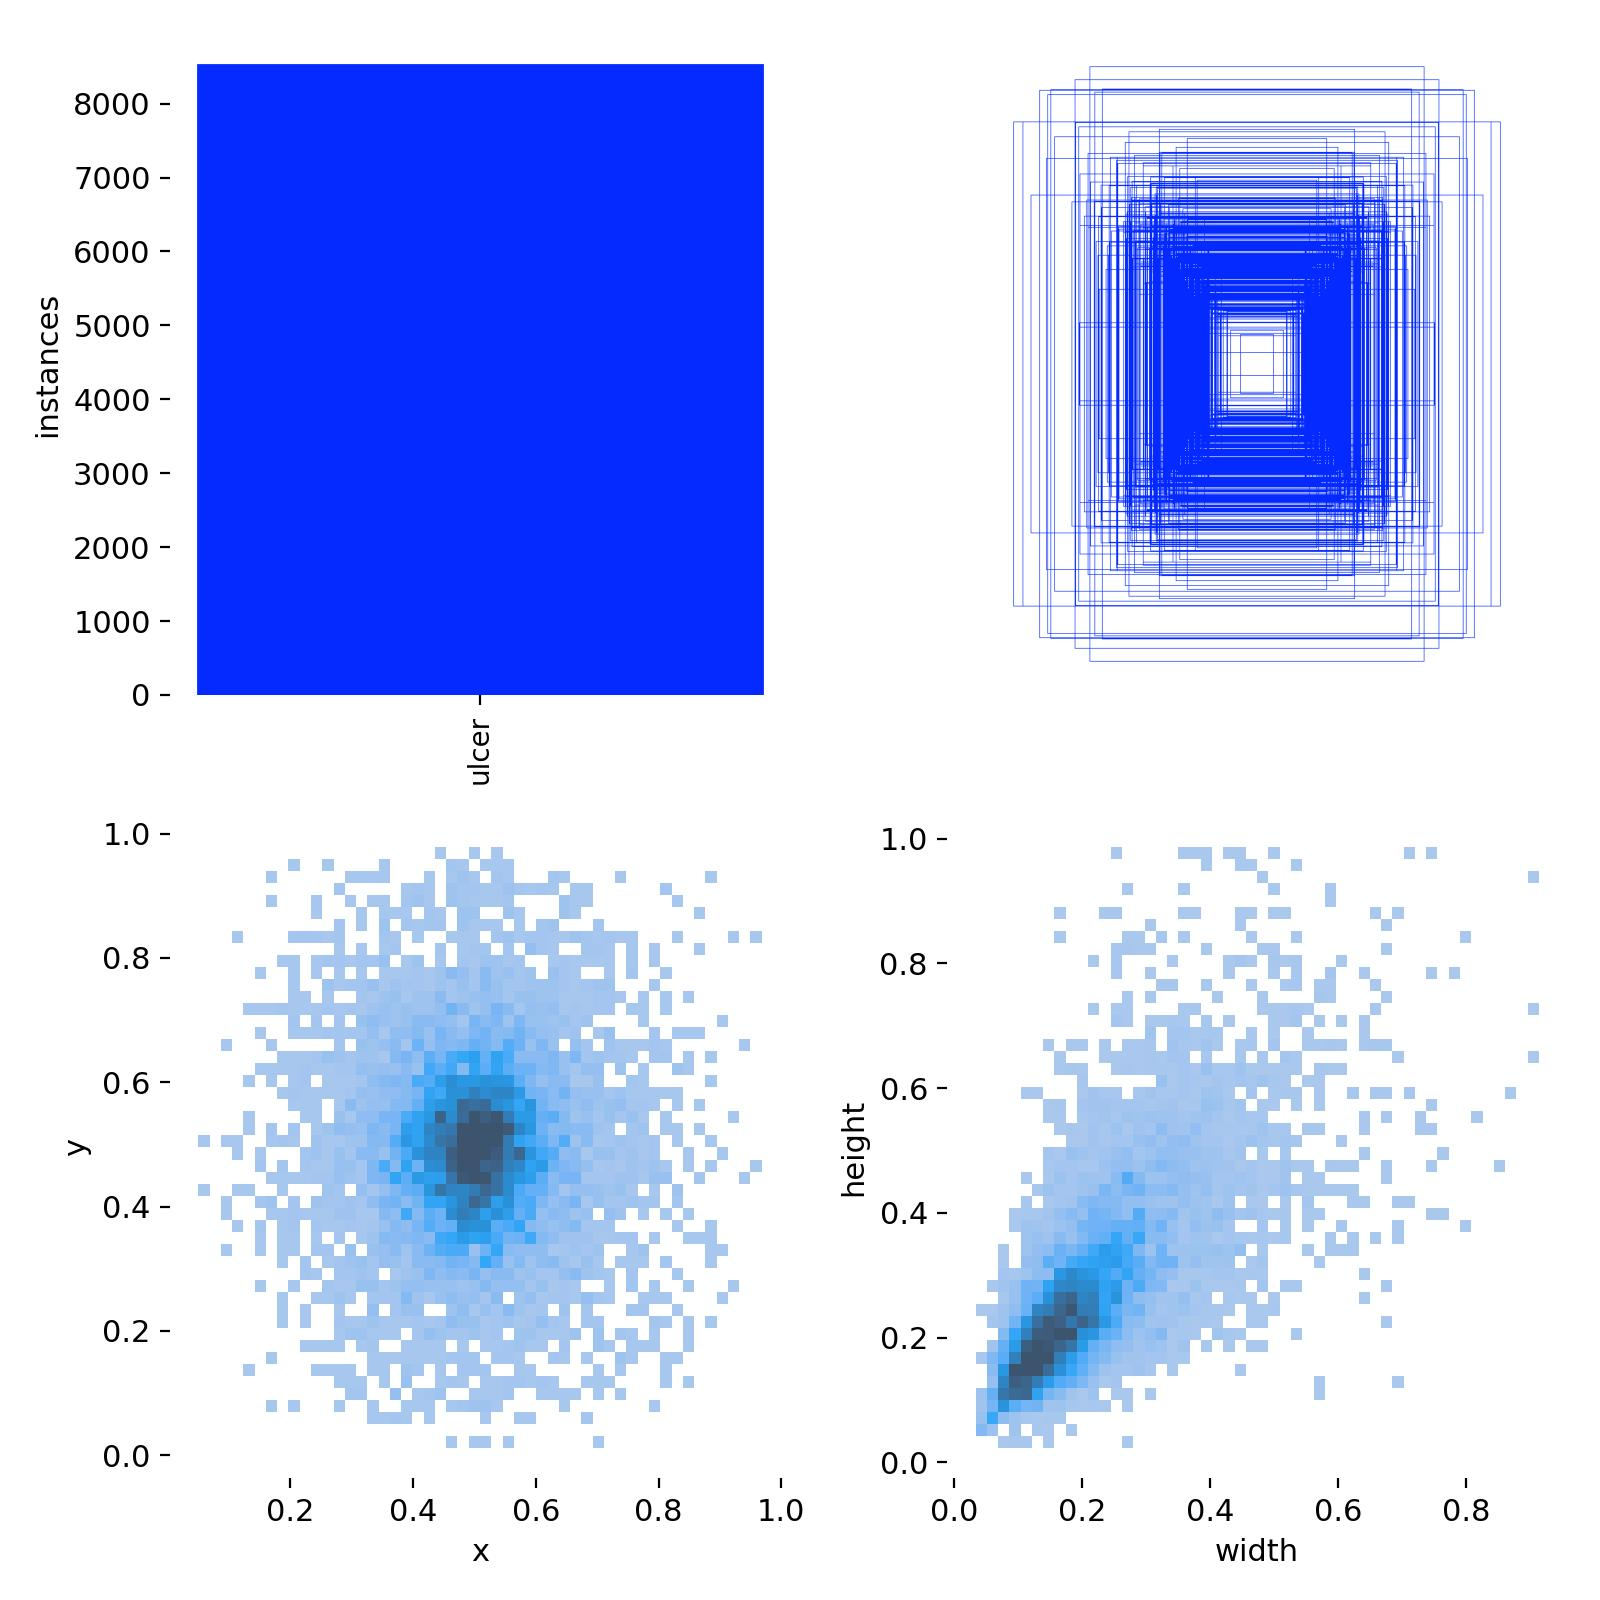
\includegraphics[width=0.85\textwidth, right]{labels.jpg}
\end{minipage}
\hfill
\begin{minipage}{0.5\textwidth}
	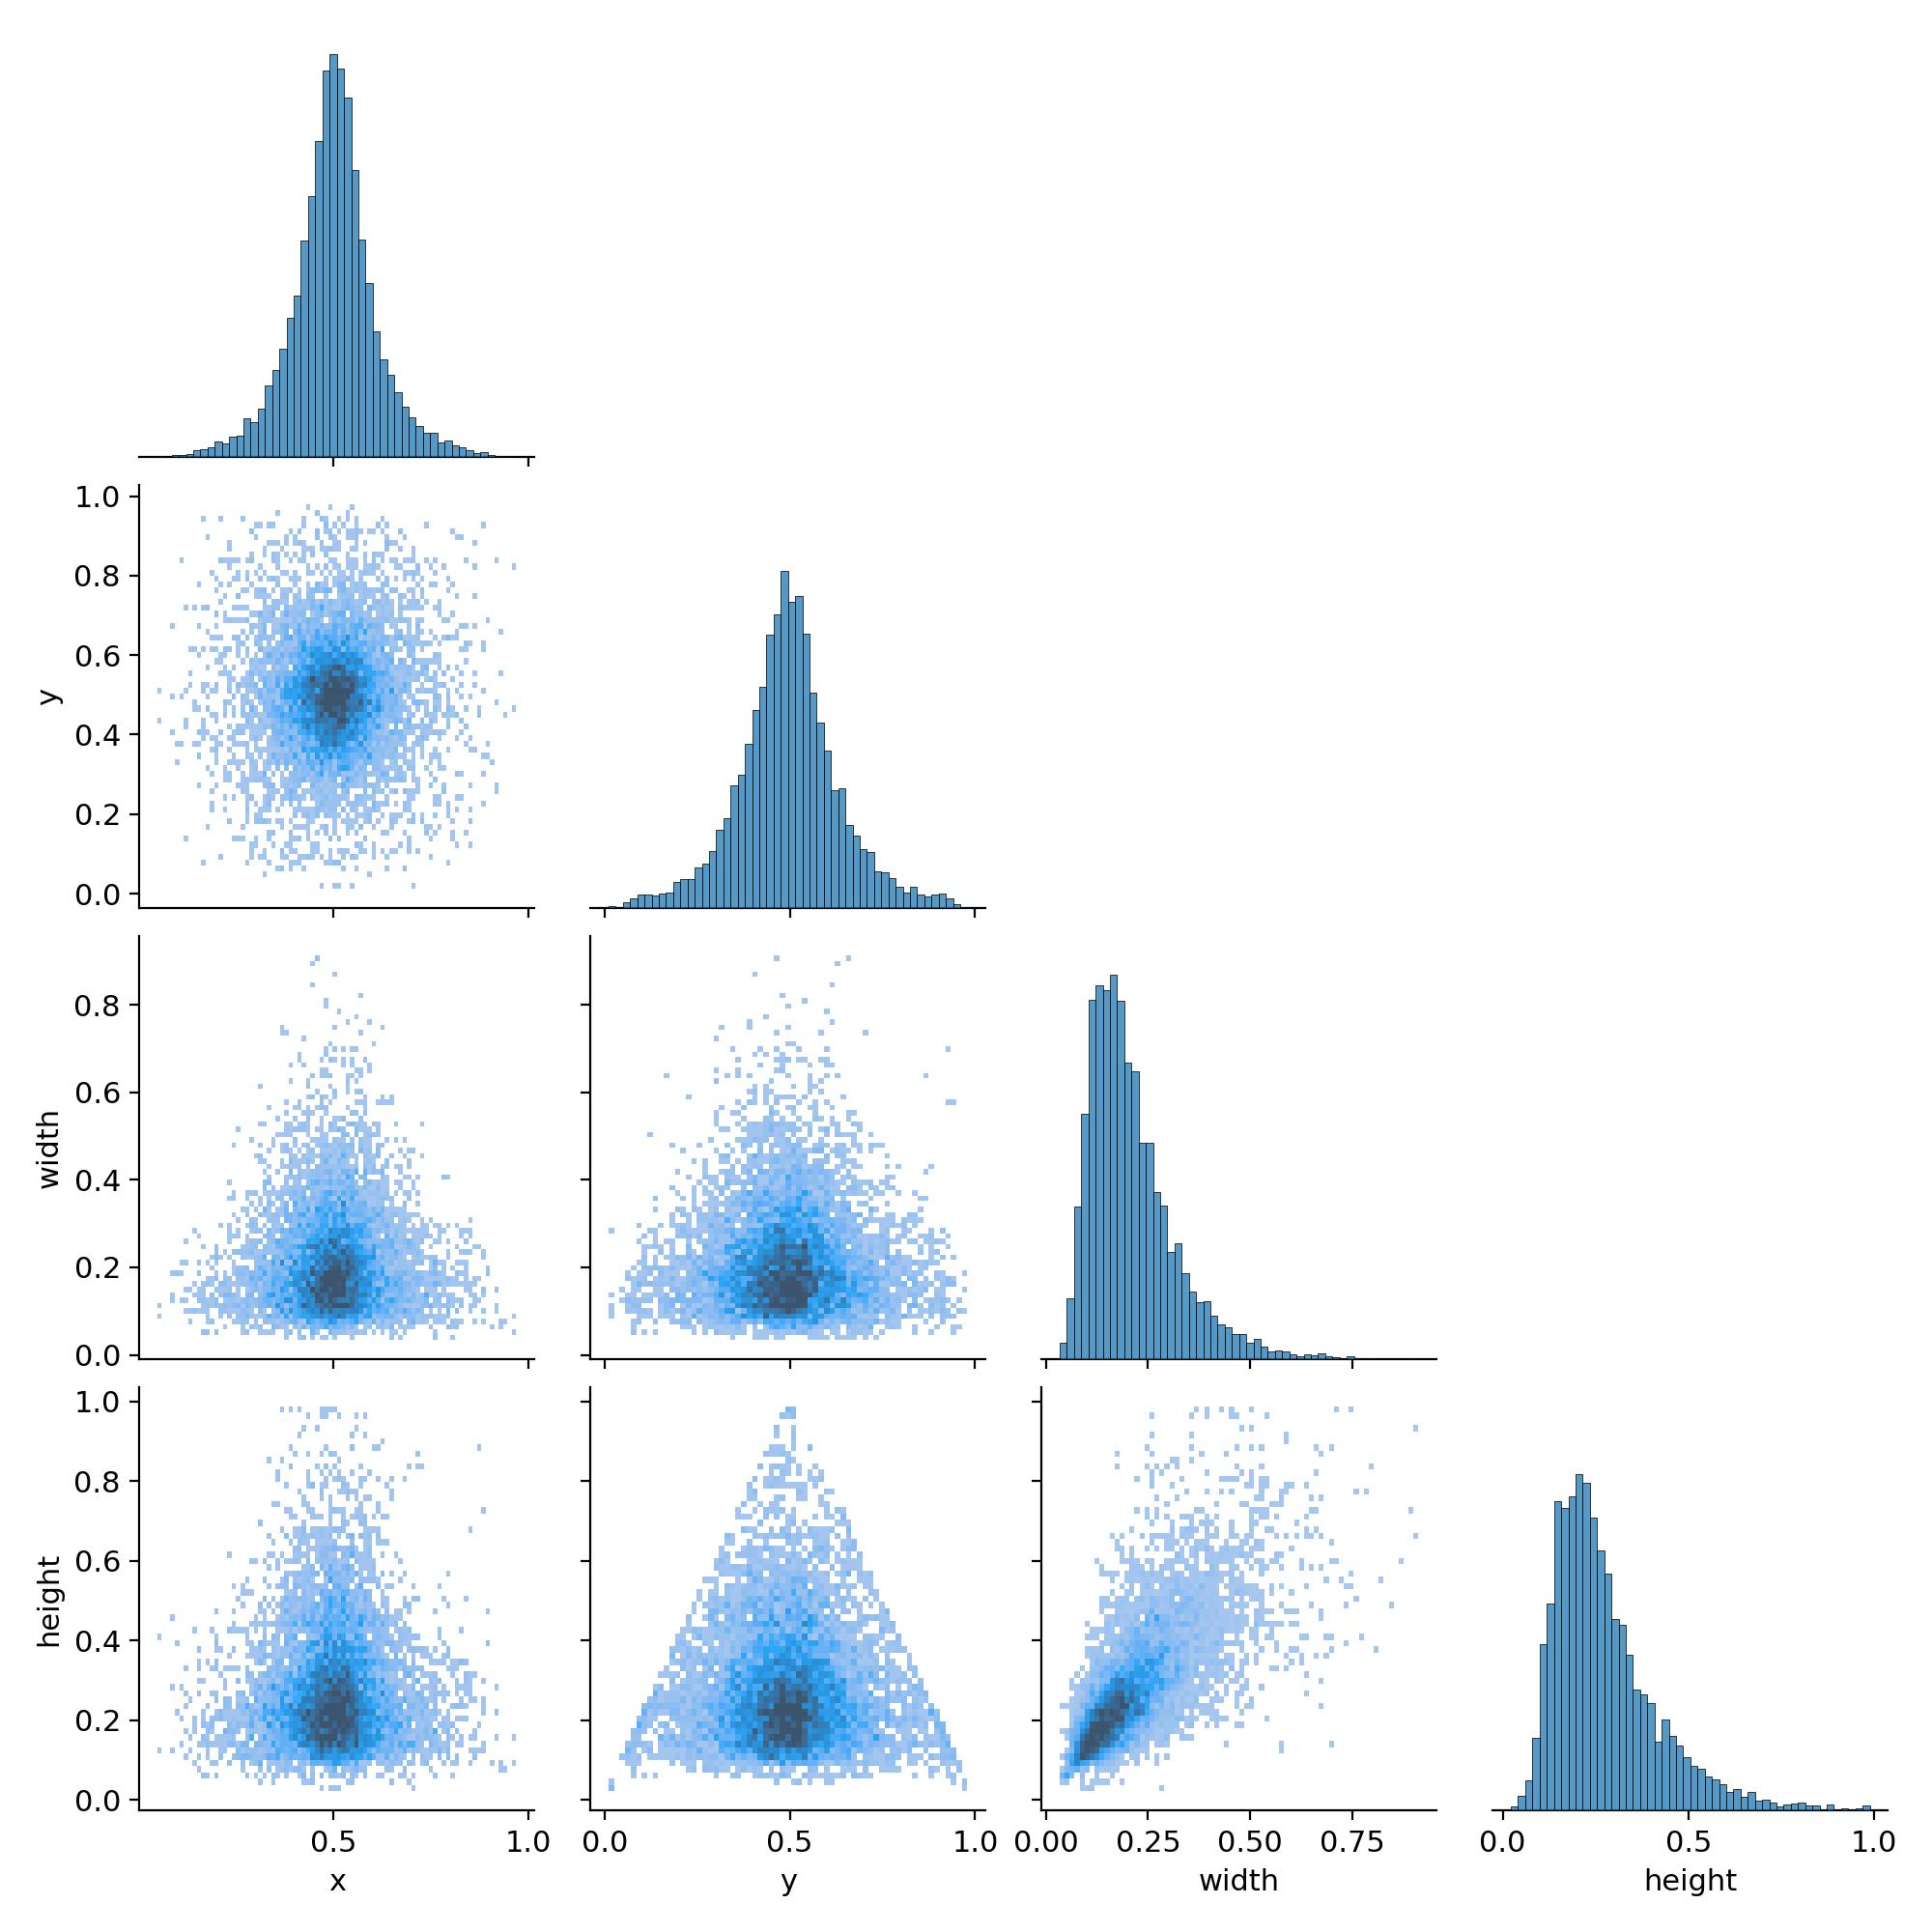
\includegraphics[width=0.7\textwidth, right]{labels_correlogram.jpg}
\end{minipage}
\gr 
\captionof{figure}{\gr Τα δεδομένα για τα \en bounding boxes \gr για όλο το \en dataset.}

\section{\gr Έλεγχος της Ποιότητας των \en Labels}
\paragraph{\textnormal{
\gr Με τη βοήθεια των συναρτήσεων \en \textbf{load\_yolo\_labels()} \gr και \en \textbf{yolo\_to\_bbox()}, \gr πραγματοποιήθηκε έλεγχος των συντεταγμένων των \en \textbf{bounding boxes}, \gr επιβεβαιώνοντας ότι όλα τα \en \textbf{label} \gr ήταν εντός των ορίων των εικόνων $(640\times 480)$. \gr Κάτα την αρχικοποίηση του \en \textbf{dataset}, \gr δεν εντοπίστηκαν ελλιπή ή κατεστραμμένα \en \textbf{annotations}.
}}

\section{\gr Αποτελέσματα ανά \en Fold (Cross-Validation)}
\paragraph{\textnormal{\gr Κατά τη συγγραφή του κώδικα χρησιμοποιήθηκε \en \textbf{5-Fold Cross-Validation} \gr ώστε να εξεταστεί η απόδοση του μοντέλου σε πολλαπλές υποδιαιρέσεις του \en \textbf{dataset}. \gr Για το κάθε \en fold \gr του κάθε μοντέλου που μελετήθηκε στην παρούσα εργασία, καταγράφηκαν οι μετρικές που παρουσιάζονται στον Πίνακα 4.1}}

\begin{table}
\centering
\renewcommand{\arraystretch}{1.5}
\begin{tabular}{|>{\columncolor[HTML]{99CC66}}p{5cm}|>{\columncolor[HTML]{99CC66}}p{10cm}|}
\hline
\en \textbf{Metric} & \en \textbf{Description} \\ \hline

\rowcolor[HTML]{E6F2DA}
\en \textbf{Precision} \gr (Ακρίβεια) & \gr Εντοπισμοί που ήταν σωστοί \en (true positives) \gr σε σχέση με όλους τους εντοπισμούς. \\ \hline

\rowcolor[HTML]{E6F2DA}
\en \textbf{Recall} \gr (Ανακλητικότητα) & \gr Σωστοί εντοπισμοί σε σχέση με όλα τα πραγματικά έλκη \en (ground truth objects). \\ \hline

\rowcolor[HTML]{E6F2DA}
\en \textbf{mAP@0.5} & \gr Μέση ακρίβεια για \en IoU > 0.5\gr . \\ \hline

\rowcolor[HTML]{E6F2DA}
\en \textbf{mAP@0.5:0.95} & \gr Μέση ακρίβεια για \en IoU \gr μεταξύ \en 0.5 \gr και \en 0.95\gr , με βήμα \en 0.05\gr . \\ \hline

\rowcolor[HTML]{E6F2DA}
\en \textbf{F1 Score} & \gr Ο μέσος όρος μεταξύ \en precision \gr και \en recall\gr , δηλαδή ο αρμονικός μέσος τους. \\ \hline

\end{tabular}
\caption{\gr \textbf{Πίνακας Μετρικών Αξιολόγησης}}
\end{table}
\section{\gr Μετρικές Αξιολόγησης)}
\paragraph{\textnormal{
\gr Για την αξιολόγηση της απόδοσης των μοντέλων, χρησιμοποιήθηκαν διάφορες μετρικές που καλύπτουν διαφορετικές πτυχές της απόδοσης, παρέχοντας μια ολοκληρωμένη εικόνα των αποτελεσμάτων. Στο κεφάλαιο αυτό θα περιγραφούν οι μετρικές που χρησιμοποιήθηκαν στην παρούσα εργασία.
}}

\section{\gr Μέθοδος Αξιολόγησης}
\paragraph{\textnormal{
\gr Για την αξιολόγηση, χρησιμοποιήθηκε \en \textbf{cross-validation} \gr στη μορφή της τεχνικής \en \textbf{k-Fold}, \gr και πιο συγκεκριμένα \en \textbf{5-Fold}, \gr όπως αναφέρθηκε και προηγουμένως. Σύμφωνα με το \en \textbf{5-Fold}, \gr τα δεδομένα χωρίζονται σε 5 τμήματα, και τα μοντέλα εκπαιδεύονται και αξιολογούνται σε κάθε τμήμα ξεχωριστά. Οι τελικές μετρήσεις προκύπτουν από τον μέσο όρο των αποτελεσμάτων όλων των \en folds. \gr Η χρήση του \en \textbf{5-Fold cross-validation} \gr επιτρέπει την πλήρη αξιοποίηση των δεδομένων και διασφαλίζει την αξιοπιστία των αποτελεσμάτων, μειώνοντας τον κίνδυνο για \en overfit \gr και παρέχοντας μια σταθερή εκτίμηση της απόδοσης των μοντέλων. 
}}
\section{\gr Μετρικές Αξιολόγησης}
\subsection{\en Accuracy}
\paragraph{\textnormal{
\gr Η ακρίβεια \en (\textbf{accuracy}) \gr υπολογίζει το ποσοστό των ορθά ταξινομημένων δειγμάτων (τόσο θετικών όσο και αρνητικών) στο σύνολο των παρατηρήσεων. Υπολογίζεται ως εξής:
\begin{center}
	$Accuracy = \frac{True Positives + True Negatives}{True Positives + True Negatives + False Positive + False Negatives}$
\end{center}
Η ακρίβεια είναι μια διαισθητική μετρική, ωστόσο μπορεί να είναι λιγότερο χρήσιμη σε περιπτώσεις μη ισορροπημένων δεδομένων, όπου η μία κλάση υπερισχύει. Για το λόγο αυτό, δεν πρέπει να λαμβάνεται υπόψιν από μόνη της. Η ακρίβεια υπολογίζεται μέσω του παρακάτω τμήματος κώδικα \cite{googleMLAccuracy} \cite{balaji2023}.
}}

\subsection{\en Precision}
\paragraph{\textnormal{
\gr Το \en \textbf{precision} \gr εστιάζει στη θετική κλάση και μετρά το πραγματικό ποσοστό των ορθών θετικών προβλέψεων σε σχέση με το συνολικό αριθμό θετικών προβλέψεων που είναι είτε \en \textbf{true} \gr είτε \en \textbf{false}:
\begin{center}
	$Precision = \frac{True Positives}{True Positives + False Positives}$
\end{center}
\gr Το \en \textbf{precision} \gr είναι σημαντικό όταν το κόστος των ψευδώς θετικών είναι υψηλό. Και σε αυτή την περίπτωση, δεν πρέπει να λαμβάνεται υπόψιν από μόνη της, αυτή η μετρική \cite{googleMLAccuracy} \cite{balaji2023}.
}}

\subsection{\en Recall}
\paragraph{\textnormal{
\gr Η μετρική \en \textbf{recall} \gr υπολογίζει το ποσοστό των πραγματικών θετικών δειγμάτων που ανιχνεύθηκαν ορθά από το μοντέλο σε σχέση με το άθροισμα των πραγματικών θετικών και των ψευδών αρνητικών:
\begin{center}
	$Recall = \frac{True Positives}{True Positives + False Negatives}$
\end{center}
\gr Η \en \textbf{recall} \gr είναι ιδιαίτερα σημαντική όταν το κόστος των ψευδώς αρνητικών είναι υψηλό \cite{googleMLAccuracy} \cite{balaji2023}.
}}

\subsection{\en F1 Score}
\paragraph{\textnormal{
\gr Στην περίπτωση εντοπισμού αντικειμένων, το \en \textbf{F1 Score} \gr υπολογίζεται ως ο αρμονικός μέσος της ακρίβειας \en (\textbf{precision}) \gr και της ανάκλησης \en (\textbf{recall}), \gr με βάση τις προβλέψεις πλαισίων \en (\textbf{bounding boxes}). \gr Μία πρόβλεψη θεωρείται ορθή \en (\textbf{true positive}) \gr όταν το \en \textbf{IoU} (Intersection over Union) \gr μεταξύ προβλεπόμενου και πραγματικού πλαισίου είναι μεγαλύτερο από ένα κατώφλι, συνήθως 0.5.
\begin{center}
	$F_{1} Score = 2 \times \frac{Precision \times Recall}{Precision + Recall}$
\end{center}
\gr Το \en \textbf{F1 Score} \gr αποτελεί έναν συνδυασμό των δύο και είναι κατάλληλη μετρική για μη ισορροπημένα δεδομένα, καθώς εξισορροπεί τις επιδόσεις μεταξύ \en \textbf{precision} \gr και \en \textbf{recall} \cite{googleMLAccuracy} \cite{balaji2023} \cite{deepchecksMetrics2023} \cite{keylabs2024}.
}}

\subsection{\en mAP Over Epochs}
\paragraph{\textnormal{
\gr Η μέση ακρίβεια εντοπισμού (\en mean Average Precision, \textbf{mAP}) \gr είναι μια βασική μετρική αξιολόγησης μοντέλων ανίχνευσης αντικειμένων. Υπολογίζει, πόσο βέλτιστα το μοντέλο προβλέπει την παρουσία και θέση των αντικειμένων σε σχέση με τα πραγματικά δεδομένα. Ο υπολογισμός της \en \textbf{mAP} \gr βασίζεται στον υπολογισμό της ακρίβειας (\en \textbf{precision}) \gr και της ανάκλησης (\en \textbf{recall}) \gr για διαφορετικά κατώφλια απόφασης. 
\gr Η ακρίβεια εκφράζει το ποσοστό των σωστών θετικών προβλέψεων επί του συνόλου των θετικών προβλέψεων, ενώ η ανάκληση μετράει το ποσοστό των σωστών θετικών προβλέψεων επί του συνόλου των πραγματικών θετικών.}}
\paragraph{\textnormal{
\gr Η \en Average Precision (\textbf{AP}) \gr υπολογίζεται ως η επιφάνεια κάτω από την καμπύλη ακρίβειας-ανάκλησης \en (\textbf{precision-recall curve}) \gr για ένα συγκεκριμένο όριο \en Intersection over Union (\textbf{IoU}), \gr δηλαδή την ελάχιστη απαιτούμενη επικάλυψη μεταξύ προβλεπόμενου και πραγματικού πλαισίου εντοπισμού.}}

\paragraph{\textnormal{
\gr Το \en \textbf{mAP} \gr προκύπτει ως ο μέσος όρος των \en \textbf{AP} \gr για όλα τα κλάσεις αντικειμένων και, συχνά, για πολλαπλά επίπεδα \en \textbf{IoU}. \gr Για παράδειγμα:
}}
\begin{itemize}
	\item \gr Το $mAP@0.5$ υπολογίζει την ακρίβεια για \en \textbf{IoU} \gr τουλάχιστον 0.5, επιτρέποντας σχετικά χαλαρή ευθυγράμμιση.
	\item \gr Το $mAP@0.5:0.95$ είναι ο μέσος όρος των \en \textbf{AP} \gr που υπολογίζονται για \en \textbf{IoU} \gr από 0.5 έως 0.95 σε βήματα 0.05, παρέχοντας πιο αυστηρή και ολοκληρωμένη αξιολόγηση.
\end{itemize}

\chapter{\gr Επιλογή Μοντέλων}
\paragraph{\textnormal{
\gr Για την παρούσα εργασία ανίχνευσης των διαβητικών ελκών ποδιού, επιλέχθηκε η χρήση μοντέλων εντοπισμού αντικειμένων \en (\textbf{object detection}) \gr βασισμένων σε τεχνολογίες \en \textbf{deep learning}. \gr Συγκεκριμένα, δοκιμάστηκαν και συγκρίθηκαν τέσσερα μοντέλα, τα οποία περιγράφονται στις παρακάτω ενότητες.}}

\section{\en YOLOv8n}
\paragraph{\textnormal{
\gr Το \en \textbf{YOLOv8n} (nano) \gr αποτελεί την πιο απλή παραλλαγή της οικογένειας \en YOLOv8, \gr  παρέχει υψηλή ταχύτητα και έχει χαμηλές απαιτήσεις υπολογιστικών πόρων. Παρότι είναι εξαιρετικά αποδοτικό σε περιβάλλοντα με περιορισμένους πόρους (π.χ. \en edge devices), \gr διατήρησε ικανοποιητική απόδοση για την ανίχνευση των ελκών. Στην εργασία αυτή αποτέλεσε αφετηρία για πειραματισμό και \en benchmarking. \cite{ultralytics}}}

\section{\en YOLOv11n}
\paragraph{\textnormal{
\gr Το \en \textbf{YOLOv11n} \gr αποτελεί μία ερευνητική παραλλαγή του \en YOLO, \gr με βελτιωμένη αρχιτεκτονική. Η εκπαίδευσή του παραγματοποιείται πιο γρήγορα σε σχέση με το \en \textbf{YOLOv8n}. \gr Παρείχε ταχύτερη σύγκλιση και σημείωσε ικανοποιητική απόδοση στις βασικές περιπτώσεις, με ελαφρώς μειωμένο \en \textbf{recall} \gr σε πιο πολύπλοκα σενάρια, για παράδειγμα σε φωτογραφίες με χαμηλή αντίθεση μεταξύ του έλκους και της υπόλοιπης εικόνας. \cite{ultralytics}}}

\section{\en YOLOv11m}
\paragraph{\textnormal{
\gr Το \en \textbf{YOLOv11m} (medium) \gr είναι μεγαλύτερο μοντέλο σε σχέση με τις \en nano \gr παραλλαγές, που αξιοποιήθηκαν στην παρούσα εργασία, και παρέχει σημαντικά βελτιωμένη ακρίβεια και ανακλητικότητα \en (\textbf{recall}). \gr Η αυξημένη χωρητικότητα του δικτύου του επιτρέπει να εντοπίζει ακόμα και μικρά ή οριακά ορατά έλκη, με υψηλή αξιοπιστία. Αποτελεί το πιο ισχυρό μοντέλο που χρησιμοποιήθηκε στη μελέτη, αν και απαιτεί μεγαλύτερους χρόνους εκπαίδευσης και μεγαλύτερη χρήση της \en GPU. \cite{ultralytics}}}

\section{\en Detectron2 R-CNN}
\paragraph{\textnormal{
\gr Το \en \textbf{Detectron2 R-CNN} \gr είναι μια σύγχρονη και ευέλικτη υλοποίηση της αρχιτεκτονικής \en R-CNN, \gr αναπτυγμένη από το \en Facebook AI Research \gr ως η επόμενη γενιά της δημοφιλούς βιβλιοθήκης \en Detectron. \gr Υποστηρίζει πολλές παραλλαγές, όπως τις \en Faster R-CNN, Mask R-CNN, Cascade R-CNN \gr και χρησιμοποιεί \en Feature Pyramid Networks (FPN) \gr για βελτιωμένη αναγνώριση αντικειμένων σε διαφορετικές κλίμακες. \gr Το \en \textbf{Detectron2} \gr βελτιώνει σημαντικά την αποδοτικότητα μέσω μοντέρνων βελτιώσεων στην αρχιτεκτονική, όπως \en batch normalization, \en multi-scale training \gr και εκμεταλλεύεται πλήρως τις δυνατότητες των σύγχρονων \en GPU \gr για ταχύτατη εκπαίδευση και \en inference. \gr Παράλληλα, διατηρεί υψηλή ακρίβεια στον εντοπισμό και την ταξινόμηση αντικειμένων, καθιστώντας το ιδανικό για ερευνητικές αλλά και βιομηχανικές εφαρμογές όπου απαιτείται αξιοπιστία και ταχύτητα. Χρησιμοποιείται συχνά ως σημείο αναφοράς για σύγκριση με άλλες σύγχρονες αρχιτεκτονικές, όπως το \en YOLO, \gr λόγω της ισορροπίας του μεταξύ απόδοσης και υπολογιστικής πολυπλοκότητας. \cite{wuDetectron22019}
}}

\chapter{\gr Βελτιστοποίηση Υπερ-παραμέτρων}
\paragraph{\textnormal{
\gr Η διαδικασία βελτιστοποίησης υπερ-παραμέτρων \en (\textbf{hyperparameter tuning}) \gr πραγματοποιήθηκε για να εξασφαλιστεί η βέλτιστη απόδοση του κάθε μοντέλου. Για το σκοπό αυτό, εφαρμόστηκε η τεχνική \en \textbf{Randomized Search Cross-Validation} \gr σε συνδυασμό με την κλιμάκωση των χαρακτηριστικών \en (\textbf{Standard Scaling}) \gr και τη μέθοδο \en \textbf{Stratified K-Fold Cross-Validation} \gr με 5 υποσύνολα.
Σε κάθε \en fold, \gr τα δεδομένα χωρίστηκαν περαιτέρω σε \en \textbf{train} \gr κατά ($90\%$) και \en \textbf{test} \gr κατά ($10\%$) με τυχαία δειγματοληψία. Αυτό διασφαλίζει την ισορροπία των κατηγοριών και την αξιοπιστία της αξιολόγησης.
}}
\section{\gr Ορισμός Υπερπαραμέτρων και Εκπαίδευσης}\vspace{-4em}
\paragraph{\textnormal{
\gr Οι υπερ-παράμετροι που επιλέχθηκαν για κάθε μοντέλο καθορίστηκαν ρητά κατά την εκπαίδευση, όπως φαίνεται στο παρακάτω απόσπασμα 6.1 του κώδικα. Οι τιμές αυτές επιλέχθηκαν βάσει βέλτιστων πρακτικών και πειραματισμού για το συγκεκριμένο πρόβλημα.
}}
\vspace{3\baselineskip}
\paragraph{}
\selectlanguage{english}
\begin{lstlisting}[caption=Training of YOLOv8 model per fold]
	model.train(
		data=yaml_path,
		epochs=60,
		imgsz=416,
		batch=16,
		project=project_dir,
		name=f'yolov11_fold{fold_num}',
		exist_ok=True,
		optimizer='SGD',
		lr0=0.01,
		patience=15,
		amp=True,
		hsv_h=0.015, hsv_s=0.7, hsv_v=0.4,
		degrees=5,
		scale=0.5,
		shear=0.1,
		perspective=0.0,
		flipud=0.0,
		fliplr=0.5,
		mosaic=0.8,
		mixup=0.0,
		copy_paste=0.0,
		auto_augment=True,
	)
\end{lstlisting}


\section{\gr Εισαγωγή Τυχαιότητας}
\paragraph{\textnormal{
\gr Παρότι δεν εφαρμόστηκε \en \textbf{explicit Randomized Search}, \gr η τυχαία δειγματοληψία των δεδομένων και η χρήση διαφορετικών \en \textbf{splits} \gr σε κάθε \en fold \gr χρησιμοποιήθηκε ως πρακτική βελτιστοποίησης, για να μειωθεί σε σχέση με το \en \textbf{ Grid Search}.
}}

\section{\gr Εκπαίδευση και Αξιολόγηση}
\paragraph{\textnormal{
\gr Σε κάθε επανάληψη του \en \textbf{cross-validation}, \gr το μοντέλο εκπαιδεύεται και αξιολογείται μετρώντας τις μετρικές, όπως αναγράφονται στο παρακάτω τμήμα κώδικα.
}}
\paragraph{}
\begin{lstlisting}
	results = model.val(iou=0.5)
	metrics = {
		'precision': float(results.box.p.mean()),
		'recall': float(results.box.r.mean()),
		'map50': float(results.box.map50.mean()),
		'map': float(results.box.map.mean()),
		'f1': float(results.box.f1.mean())
	}
\end{lstlisting}
\paragraph{\textnormal{
\gr Τα αποτελέσματα του κάθε \en fold \gr αποθηκεύονται σε μία λίστα αρχικά και τελικά σε ένα αρχείο \en \textbf{csv}.	
}}
\paragraph{}
\begin{lstlisting}
	df = pd.DataFrame(fold_results)
	df.loc['Mean'] = df.mean(numeric_only=True)
	df.to_csv(results_csv, index=False)
\end{lstlisting}
\paragraph{\textnormal{
\gr Έτσι διασφαλίζεται η αναλυτική καταγραφή των αποτελεσμάτων και η δυνατότητα σύγκρισης.
}}
\begin{center}
	\begin{tabular}{|c|c|c|c|c|c|}
		\hline
		\cellcolor[HTML]{CCE5E5} \textbf{Fold} & \cellcolor[HTML]{CCE5E5} \textbf{Precision} & \cellcolor[HTML]{CCE5E5} \textbf{Recall} & \cellcolor[HTML]{CCE5E5} \textbf{mAP@0.5} & \cellcolor[HTML]{CCE5E5} \textbf{mAP@0.5:0.95} & \cellcolor[HTML]{CCE5E5} \textbf{F1} \\
		\hline
		\cellcolor[HTML]{FFE0CC} 1 & \cellcolor[HTML]{E6F2E6} 0.7756 & \cellcolor[HTML]{E6F2E6} 0.6999 & \cellcolor[HTML]{E6F2E6} 0.7562 & \cellcolor[HTML]{E6F2E6} 0.3363 & \cellcolor[HTML]{FFE0CC} 0.7358 \\
		\hline
		\cellcolor[HTML]{FFE0CC} 2 & \cellcolor[HTML]{E6F2E6} 0.7711 & \cellcolor[HTML]{E6F2E6} 0.6803 & \cellcolor[HTML]{E6F2E6} 0.7551 & \cellcolor[HTML]{E6F2E6} 0.3364 & \cellcolor[HTML]{FFE0CC} 0.7228 \\
		\hline
		\cellcolor[HTML]{FFE0CC} 3 & \cellcolor[HTML]{E6F2E6} 0.8004 & \cellcolor[HTML]{E6F2E6} 0.6895 & \cellcolor[HTML]{E6F2E6} 0.7674 & \cellcolor[HTML]{E6F2E6} 0.3352 & \cellcolor[HTML]{FFE0CC} 0.7408 \\
		\hline
		\cellcolor[HTML]{FFE0CC} 4 & \cellcolor[HTML]{E6F2E6} 0.7920 & \cellcolor[HTML]{E6F2E6} 0.6717 & \cellcolor[HTML]{E6F2E6} 0.7499 & \cellcolor[HTML]{E6F2E6} 0.3346 & \cellcolor[HTML]{FFE0CC} 0.7269 \\
		\hline
		\cellcolor[HTML]{FFE0CC} 5 & \cellcolor[HTML]{E6F2E6} 0.7829 & \cellcolor[HTML]{E6F2E6} 0.7048 & \cellcolor[HTML]{E6F2E6} 0.7712 & \cellcolor[HTML]{E6F2E6} 0.3403 & \cellcolor[HTML]{FFE0CC} 0.7418 \\
		\hline
		\cellcolor[HTML]{FFE0CC} Avg (Fold 3×2) & \cellcolor[HTML]{E6F2E6} 0.7844 & \cellcolor[HTML]{E6F2E6} 0.6892 & \cellcolor[HTML]{E6F2E6} 0.7600 & \cellcolor[HTML]{E6F2E6} 0.3366 & \cellcolor[HTML]{FFE0CC} 0.7336 \\
		\hline
	\end{tabular}
	\gr 
	\captionof{table}{\gr Αρχείο \en csv \gr για το μοντέλο \en YOLOv8n}
\end{center}
\section{\gr Επιλογή Καλύτερων Μοντέλων}
\paragraph{\textnormal{
\gr Τα βάρη του καλύτερου μοντέλου για κάθε \en fold \gr αποθηκεύονται ξεχωριστά.}}
\paragraph{}
\begin{lstlisting}
	best_weights = (
		f"{project_dir}/yolov11_fold{fold_num}/weights/best.pt"
	)
	shutil.copy(
		best_weights,
		f"{project_dir}/yolov11_fold{fold_num}_best.pt"
	)
\end{lstlisting}

\paragraph{\textnormal{
\gr Με αυτόν τον τρόπο, τα μοντέλα με την καλύτερη απόδοση είναι δυνατό να διατηρηθούν για περαιτέρω ανάλυση. Συνολικά, η διαδικασία αποτυπώθηκε με τέτοιο τρόπο ώστε να περιλαμβάνονται οι αναλυτικές μετρήσεις για κάθε \en fold, \gr καθώς και οι καλύτεροι συνδυασμοί υπερ-παραμέτρων, όπως φαίνεται στα αποθηκευμένα \en csv \gr αρχεία.
}}
\gr

\chapter{\gr Μέθοδος και Μετρικές Αξιολόγησης}
\paragraph{\textnormal{
\gr Για την αξιολόγηση της απόδοσης των μοντέλων, χρησιμοποιήθηκαν διάφορες μετρικές που καλύπτουν διαφορετικές πτυχές της απόδοσης, παρέχοντας μια ολοκληρωμένη εικόνα των αποτελεσμάτων. Στο κεφάλαιο αυτό θα περιγραφούν οι μετρικές που χρησιμοποιήθηκαν στην παρούσα εργασία.
}}

\section{\gr Μέθοδος Αξιολόγησης}
\paragraph{\textnormal{
\gr Για την αξιολόγηση του μοντέλου, χρησιμοποιήθηκε \en \textbf{cross-validation} \gr στη μορφή της τεχνικής \en \textbf{k-Fold}, \gr και πιο συγκεκριμένα \en \textbf{5-Fold}, \gr όπως αναφέρθηκε και προηγουμένως. Σύμφωνα με το \en \textbf{5-Fold}, \gr τα δεδομένα χωρίζονται σε 5 τμήματα, και το μοντέλο εκπαιδεύεται και αξιολογείται σε κάθε τμήμα ξεχωριστά. Οι τελικές μετρήσεις προκύπτουν από τον μέσο όρο των αποτελεσμάτων όλων των \en folds. \gr Η χρήση του \en \textbf{5-Fold cross-validation} \gr επιτρέπει την πλήρη αξιοποίηση των δεδομένων και διασφαλίζει την αξιοπιστία των αποτελεσμάτων, μειώνοντας τον κίνδυνο για \en overfit \gr και παρέχοντας μια σταθερή εκτίμηση της απόδοσης του μοντέλου. 
}}
\section{\gr Μετρικές Αξιολόγησης}
\subsection{\en Accuracy}
\paragraph{\textnormal{
\gr Η ακρίβεια \en (\textbf{accuracy}) \gr υπολογίζει το ποσοστό των ορθά ταξινομημένων δειγμάτων (τόσο θετικών όσο και αρνητικών) στο σύνολο των παρατηρήσεων. Υπολογίζεται ως εξής:
\begin{center}
	$Accuracy = \frac{True Positives + True Negatives}{True Positives + True Negatives + False Positive + False Negatives}$
\end{center}
Η ακρίβεια είναι μια διαισθητική μετρική, ωστόσο μπορεί να είναι λιγότερο χρήσιμη σε περιπτώσεις μη ισορροπημένων δεδομένων, όπου η μία κλάση υπερισχύει. Για το λόγο αυτό, δεν πρέπει να λαμβάνεται υπόψιν από μόνη της. Η ακρίβεια υπολογίζεται μέσω του παρακάτω τμήματος κώδικα \cite{googleMLAccuracy} \cite{balaji2023}.
}}

\subsection{\en Precision}
\paragraph{\textnormal{
\gr Το \en \textbf{precision} \gr εστιάζει στη θετική κλάση και μετρά το πραγματικό ποσοστό των ορθών θετικών προβλέψεων σε σχέση με το συνολικό αριθμό θετικών προβλέψεων που είναι είτε \en \textbf{true} \gr είτε \en \textbf{false}:
\begin{center}
	$Precision = \frac{True Positives}{True Positives + False Positives}$
\end{center}
\gr Το \en \textbf{precision} \gr είναι σημαντικό όταν το κόστος των ψευδώς θετικών είναι υψηλό. Και σε αυτή την περίπτωση, δεν πρέπει να λαμβάνεται υπόψιν από μόνη της, αυτή η μετρική \cite{googleMLAccuracy} \cite{balaji2023}.
}}

\subsection{\en Recall}
\paragraph{\textnormal{
\gr Η μετρική \en \textbf{recall} \gr υπολογίζει το ποσοστό των πραγματικών θετικών δειγμάτων που ανιχνεύθηκαν ορθά από το μοντέλο σε σχέση με το άθροισμα των πραγματικών θετικών και των ψευδών αρνητικών:
\begin{center}
	$Recall = \frac{True Positives}{True Positives + False Negatives}$
\end{center}
\gr Η \en \textbf{recall} \gr είναι ιδιαίτερα σημαντική όταν το κόστος των ψευδώς αρνητικών είναι υψηλό \cite{googleMLAccuracy} \cite{balaji2023}.
}}

\subsection{\en F1 Score}
\paragraph{\textnormal{
\gr Στην περίπτωση εντοπισμού αντικειμένων, το \en \textbf{F1 Score} \gr υπολογίζεται ως ο αρμονικός μέσος της ακρίβειας \en (\textbf{precision}) \gr και της ανάκλησης \en (\textbf{recall}), \gr με βάση τις προβλέψεις πλαισίων \en (\textbf{bounding boxes}). \gr Μία πρόβλεψη θεωρείται ορθή \en (\textbf{true positive}) \gr όταν το \en \textbf{IoU} (Intersection over Union) \gr μεταξύ προβλεπόμενου και πραγματικού πλαισίου είναι μεγαλύτερο από ένα κατώφλι, συνήθως 0.5.
\begin{center}
	$F_{1} Score = 2 \times \frac{Precision \times Recall}{Precision + Recall}$
\end{center}
\gr Το \en \textbf{F1 Score} \gr αποτελεί έναν συνδυασμό των δύο και είναι κατάλληλη μετρική για μη ισορροπημένα δεδομένα, καθώς εξισορροπεί τις επιδόσεις μεταξύ \en \textbf{precision} \gr και \en \textbf{recall} \cite{googleMLAccuracy} \cite{balaji2023} \cite{deepchecksMetrics2023} \cite{keylabs2024}.
}}



\begin{thebibliography}{8}
\en 
\bibitem{frontiers2022} 
G. V. Georgoulas, A. T. Tzallas, D. I. Fotiadis, and M. Tsipouras, 
\textit{A review of non-invasive sensors and artificial intelligence models for diabetic foot monitoring}, 
Frontiers in Physiology, vol. 13, 2022. DOI: \url{https://doi.org/10.3389/fphys.2022.924546}.
\en 
\bibitem{wagner2022} 
S. B. Reddy, A. K. Jadhav, and S. S. Reddy, 
\textit{Wagner's Classification as a Tool for Treating Diabetic Foot Ulcers: Our Observations at a Suburban Teaching Hospital}, 
Cureus, vol. 14, no. 2, 2022. DOI: \url{https://doi.org/10.7759/cureus.22492}.

\bibitem{dfu_classifications_review} 
S. M. Abolarinwa, 
\textit{Diabetic foot ulcer classifications: A critical review}, 
International Journal of Diabetes and Clinical Research, vol. 5, no. 2, pp. 1-6, 2018. DOI: \url{https://doi.org/10.23937/2377-3634/1410085}.

\bibitem{dfu_risk_factors_management} 
A. A. Al-Rubeaan, 
\textit{Diabetic foot ulcers: Classification, risk factors and management}, 
Saudi Journal of Biological Sciences, vol. 26, no. 7, pp. 1403-1411, 2019. DOI: \url{https://doi.org/10.1016/j.sjbs.2019.06.002}.

\bibitem{telemedical_monitoring} 
M. K. Wurdemann et al., 
\textit{Hospital stays and costs of telemedical monitoring versus standard follow-up for diabetic foot ulcer: an open-label randomised controlled study}, 
The Lancet Regional Health – Europe, vol. 3, 2021. DOI: \url{https://doi.org/10.1016/j.lanepe.2021.100053}.

\bibitem{ai_dfu_detection} 
M. H. Yap et al., 
\textit{Artificial intelligence for automated detection of diabetic foot ulcers: A real-world proof-of-concept clinical evaluation}, 
Diabetes Research and Clinical Practice, vol. 165, 2020. DOI: \url{https://doi.org/10.1016/j.diabres.2020.108252}.

\bibitem{ml_dfu_review} 
S. K. Mishra et al., 
\textit{The role of machine learning in advancing diabetic foot: a review}, 
Frontiers in Endocrinology, vol. 12, 2021. DOI: \url{https://doi.org/10.3389/fendo.2021.708433}.

\bibitem{ai_clinical_prediction} 
J. W. Su et al., 
\textit{Updating methods for artificial intelligence-based clinical prediction models: a scoping review}, 
BMJ Open, vol. 11, no. 5, 2021. DOI: \url{https://doi.org/10.1136/bmjopen-2020-045202}.

\bibitem{sarmun2024diabetic} 
R. Sarmun et al., 
\textit{Diabetic Foot Ulcer Detection: Combining Deep Learning Models for Improved Localization}, 
Cognitive Computation, vol. 16, no. 6, pp. 1413--1431, 2024. DOI: \url{https://doi.org/10.1007/s12559-024-10267-3}.

\bibitem{dfu_dataset} 
Roboflow,  
\textit{Diabetic Foot Ulcer Dataset},  
Available at: \url{https://universe.roboflow.com/my-datasets-g2gqc/diabetic-foot-ulcer/dataset/6}.

\bibitem{ultralytics}
Ultralytics. (2024). YOLOv8 Documentation. 
Retrieved from \url{https://docs.ultralytics.com}

\bibitem{roboflow}
The dataset used for this assignment was retrieved from: \url{https://universe.roboflow.com/my-datasets-g2gqc/diabetic-foot-ulcer/dataset/6}

\bibitem{roboflowrcnn}
Roboflow. (2023). What is R-CNN?  
Retrieved from \url{https://blog.roboflow.com/what-is-r-cnn/}

\bibitem{googleMLAccuracy} 
Google Developers, 
\textit{Classification: Accuracy, Precision, Recall}, 
Machine Learning Crash Course, 2023. 
Available at: \url{https://developers.google.com/machine-learning/crash-course/classification/accuracy-precision-recall}

\bibitem{balaji2023}
Balaji G., 
\textit{Mastering Classification Metrics: A Deep Dive from F1 Score to AUC-ROC}, 
Medium, 2023. 
Available at: \url{https://medium.com/@balaji92/mastering-classification-metrics-a-deep-dive-from-f1-score-to-auc-roc-87e82b0ebfae}

\bibitem{deepchecksMetrics2023}
Deepchecks,
\textit{Understanding F1 Score, Accuracy, ROC-AUC \& PR-AUC Metrics},
2023.
Available at: \url{https://www.deepchecks.com/f1-score-accuracy-roc-auc-and-pr-auc-metrics-for-models/}

\bibitem{keylabs2024}
Keylabs,
\textit{Understanding the F1 Score and AUC-ROC Curve},
October 25, 2024.
Available at: \url{https://keylabs.ai/blog/understanding-the-f1-score-and-auc-roc-curve/}

\bibitem{neptuneMetrics2022}
Neptune.ai,
\textit{F1 Score vs ROC AUC vs Accuracy vs PR AUC: Which Evaluation Metric Should You Choose?},
2022.
Available at: \url{https://neptune.ai/blog/f1-score-accuracy-roc-auc-pr-auc}

\bibitem{datacampAUC2024}
Kurtis Pykes,
\textit{AUC and the ROC Curve in Machine Learning},
DataCamp, September 10, 2024.
Available at: \url{https://www.datacamp.com/tutorial/auc}

\bibitem{wuDetectron22019}
Yuxin Wu, Alexander Kirillov, Francisco Massa, Wan-Yen Lo, and Ross Girshick,  
\textit{Detectron2},  
Facebook AI Research, October 2019.  
Available at: \url{https://github.com/facebookresearch/detectron2}


\end{thebibliography}




\end{document}
